% -*-coding: utf-8-*-
% This is an AMS-LaTeX v. 1.2 File.

\documentclass{report}

%\usepackage{pscyr}
%\renewcommand{\rmdefault}{fjn}
%\renewcommand{\ttdefault}{fcr}

%\usepackage{showkeys}
\usepackage{cmap}
\usepackage[T2A]{fontenc}
\usepackage[utf8x]{inputenc}
\usepackage[english,russian]{babel}
\usepackage{expdlist}
\usepackage[pdftex]{graphicx}
\usepackage{amsmath}
\usepackage{amssymb}
\usepackage{amsthm}
\usepackage{amsfonts}
\usepackage{amsxtra} 
\usepackage{array}
\usepackage{wrapfig}
\usepackage{sty/dbl12}
\usepackage{srcltx}
\usepackage{epsfig}
\usepackage{verbatim}
\usepackage{sty/rac}
%\usepackage[russian]{sty/ralg}

\usepackage{xspace}
\usepackage{algorithm}
\usepackage{algorithmicx}
\usepackage{algpseudocode}


\usepackage{listings}
\usepackage{placeins}
\usepackage{caption}
\usepackage{subfigure}
\usepackage{easytable}
%\usepackage{floatrow}
\captionsetup[table]{position=t,justification=raggedright,slc=off}

\def\BState{\State\hskip-\ALG@thistlm}
\makeatother

%\usepackage[
%    top    = 2.00cm,
%    bottom = 2.00cm,
%    left   = 3.00cm,
%    right  = 1.50cm]{geometry}
\hoffset = -10mm
\voffset = -20mm
\textheight = 230mm
\textwidth = 165mm

%%%%%%%%%%%%%%%%%%%%%%%%%%%%%%%%%%%%%%%%%%%%%%%%%%%%%%%%%%%%%%%%%%%%%%%%%%%%%%

% Redefine margins and other page formatting

%\setlength{\oddsidemargin}{0.5in}

% Various theorem environments. All of the following have the same numbering
% system as theorem.

\theoremstyle{plain}
\newtheorem{theorem}{Теорема}
\newtheorem{prop}[theorem]{Утверждение}
\newtheorem{corollary}[theorem]{Следствие}
\newtheorem{lemma}[theorem]{Лемма}
\newtheorem{question}[theorem]{Вопрос}
\newtheorem{conjecture}[theorem]{Гипотеза}
\newtheorem{assumption}[theorem]{Предположение}

\theoremstyle{definition}
\newtheorem{definition}[theorem]{Определение}
\newtheorem{notation}[theorem]{Обозначение}
\newtheorem{condition}[theorem]{Условие}
\newtheorem{example}[theorem]{Пример}
%\newtheorem{algorithm}[theorem]{Алгоритм}
%\newtheorem{introduction}[theorem]{Introduction}

\newtheorem{algo}[theorem]{Алгоритм}

\floatname{algorithm}{Алгоритм}

\algnewcommand\algorithmicand{\textbf{and}\xspace}
\algnewcommand\algorithmicor{\textbf{or}\xspace}
\algnewcommand\algorithmicnot{\textbf{not}\xspace}
\algnewcommand\algorithmictrue{\textbf{true}}
\algnewcommand\algorithmicfalse{\textbf{false}}
\algtext*{EndWhile} % Remove "end while" text
\algtext*{EndIf} % Remove "end if" text
\algtext*{EndFor} % Remove "end for" text
\algtext*{EndProcedure} % Remove "end for" text

\renewcommand{\proof}{\\\textbf{Доказательство.}~}

%\def\startprog{\begin{lstlisting}[language=Java,basicstyle=\normalsize\ttfamily]}

%\theoremstyle{remark}
%\newtheorem{remark}[theorem]{Remark}
%\include{header}
%%%%%%%%%%%%%%%%%%%%%%%%%%%%%%%%%%%%%%%%%%%%%%%%%%%%%%%%%%%%%%%%%%%%%%%%%%%%%%%

\numberwithin{theorem}{chapter}        % Numbers theorems "x.y" where x
                                        % is the section number, y is the
                                        % theorem number

%\renewcommand{\thetheorem}{\arabic{chapter}.\arabic{theorem}}

%\makeatletter                          % This sequence of commands will
%\let\c@equation\c@theorem              % incorporate equation numbering
%\makeatother                           % into the theorem numbering scheme

%\renewcommand{\theenumi}{(\roman{enumi})}

%%%%%%%%%%%%%%%%%%%%%%%%%%%%%%%%%%%%%%%%%%%%%%%%%%%%%%%%%%%%%%%%%%%%%%%%%%%%%%


%%%%%%%%%%%%%%%%%%%%%%%%%%%%%%%%%%%%%%%%%%%%%%%%%%%%%%%%%%%%%%%%%%%%%%%%%%%%%%%

%This command creates a box marked ``To Do'' around text.
%To use type \todo{  insert text here  }.

\newcommand{\todo}[1]{\vspace{5 mm}\par \noindent
\marginpar{\textsc{ToDo}}
\framebox{\begin{minipage}[c]{0.95 \textwidth}
\tt #1 \end{minipage}}\vspace{5 mm}\par}

%%%%%%%%%%%%%%%%%%%%%%%%%%%%%%%%%%%%%%%%%%%%%%%%%%%%%%%%%%%%%%%%%%%%%%%%%%%%%%%

\binoppenalty=10000
\relpenalty=10000

\begin{document}

% Begin the front matter as required by Rackham dissertation guidelines

\initializefrontsections

\pagestyle{title}

\begin{center}
Санкт-Петербургский национальный исследовательский университет \\ информационных технологий, механики и оптики

\vspace{2cm}

Кафедра компьютерных технологий

\vspace{3cm}

{\Large Минаев Б. Ю.}

\vspace{2cm}

\vbox{\LARGE\bfseries
Реализация динамических Rake-Compress деревьев в случае отсутствия ограничения на степени вершин}

\vspace{4cm}

Бакалаврская работа 

\vspace{1cm}

{\Large Научный руководитель: Буздалов М. В.}

\vspace{5cm}

Санкт-Петербург\\ 2015
\end{center}

\newpage

\setcounter{page}{4}
\pagestyle{plain}

%\dedicationpage{Put a dedication here}
% Dedication page

%\startacknowledgementspage
% Acknowledgements page
%{Put Acknowledgements here}

% Table of contents, list of figures, etc.
\tableofcontents
%\listoffigures


\def\t#1{\mbox{\texttt{\hbox{#1}}}}
\def\b#1{\textbf{#1}}
\def\tb#1{\t{\b{#1}}}

\def\cln#1{\t{#1}}
\def\pcn#1{\t{#1}}
\newcommand{\p}{\par Здесь будет текст...}
\def\putImgx#1#2{
  \includegraphics[width=#1]{../img/#2}
}

\def\putImg#1{
  \includegraphics{../img/#1}
}

\def\drawfigure#1#2{
        \begin{figure}
        \putImg{#1}
        \caption{#2}
        \label{#1}
        \end{figure}
}
\def\drawfigurex#1#2#3#4{
        \begin{figure}[ht]
          \begin{center}
            \putImgx{#4}{#1}
            \caption{#2}
            \label{#3}
          \end{center}
        \end{figure}
}
 
% Chapters
\startthechapters
% -*-coding: utf-8-*-
\startprefacepage

Динамические деревья находят множество применений в области информационных технологий. В частности, они используются в 
алгоритмах поиска максимального потока, а также для решения задачи динамической 
связности ациклических графов. Например, они позволяют уменьшить время работы алгоритма проталкивания
предпотока с $O(EV^2)$ до $O(EV \log (V^2 / E))$~\cite{tarj86}. 

Зачастую, термин <<динамические деревья>> ассоциируется только с Link-Cut деревьями, которые были предложены 
Слетером и Тарьяном~\cite{tarj83}. Однако существуют и другие динамические деревья: например, Top-деревья~\cite{alst05} и Rake-Compress деревья~\cite{acar04, acar05}.
В данной работе рассмотрены именно последние. Они обладают существенным преимуществом перед другими динамическими 
деревьями --- их построение можно сделать параллельным.

На сегодняшний день большинство процессоров содержат несколько ядер, способных работать параллельно. 
Поэтому актуальной задачей является разработка алгоритмов, способных работать на нескольких ядрах одновременно.
Алгоритмы, базирующиеся на Rake-Compress деревьях, являются таковыми.

Реализация Rake-Compress деревьев, которая была предложена Умутом Акаром в оригинальной статье~\cite{acar04} обладала несколькими недостатками:
\begin{itemize}
\item Рассматривались только деревья, у которых степень каждой вершины ограничена некоторой константой. 
\item Статья носит скорее теоретический, нежели практический характер. В ней уделяется внимание только асимптотическим оценкам. 
На практике же необходимо иметь структуры данных, эффективные не только асимптотически, но и с точки зрения времени работы на реальных данных. 
\end{itemize}

В данной работе показано как избавиться от ограничения на степени вершин, а также как эффективно реализовывать Rake-Compress деревья.

\FloatBarrier

%-*-coding: utf-8-*-
\chapter{Обзор динамических деревьев}
\label{chapSVD}

В данной главе рассмотрены необходимые понятия теории графов, 
определена задача, которая решается с помощью динамических деревьев, 
описаны области, в которых они приминимы, а также 
приведен краткий обзор существующих динамических деревьев. 
В главе также выделены проблемы Rake-Compress деревьев, решению которых посвещена данная работа.

\section{Необходимые элементы теории графов}

Для начала введем несколько определений из теории графов, которые понадобятся в работе.

{\bf Графом} называется упорядоченная пара $(V, E)$, где $V$ --- множество вершин, а $E$ --- множество ребер.

Различают {\bf ориентированные} и {\bf неориентированные} графы. В первом случае каждое ребро это упорядоченная пара вершин, во втором --- неупорядоченная.

Вершина $v$ является {\bf смежной} с $u$, если в графе существует ребро $(u, v)$.

Говорят, что из $u$ {\bf достижима} $v$, если существует список вершин такой, что:
\begin{itemize}
\item первая вершина в списке --- $u$
\item последняя вершина в списке --- $v$
\item соседние вершины списка являются смежными
\end{itemize}  

Граф называется {\bf связным}, если для любой пары вершин $(u, v)$ $u$ достижима из $v$.

{\bf Деревом} называется связный неориентированный граф с $n$ вершинами и $n - 1$ ребром.

{\bf Степенью вершины} называется количество вершин, которые смежны с данной. В случае ориентированных графов различают {\bf входящую} и {\bf исходящую} степень. 

{\bf Корневым деревом} называется граф с выделенной вершиной --- корнем. Исходящая степень корня равна нулю, а исходящая степень любой другой вершины --- единице. Корень должен быть достижим из всех вершин.

{\bf Поддеревом} вершины $v$ называется множество всех вершин, из которых достижима $v$.

{\bf Листом} называется вершина, входящая степень которой равна нулю.

{\bf Лесом} называется множество деревьев, которые не пересекаются по вершинам.

В данной работе большинство внимания уделено эффективному хранению леса, каждое дерево которого является корневым. 
Однако, в разделе \ref{sec:undirected} рассмотрен случай неориентированных деревьев.

\FloatBarrier

\section{Динамические деревья}

Задача, которая решается с помощью динамических деревьев, формулируется следующим образом. Необходимо поддерживать лес деревьев и выполнять на нем следующие операции:
\begin{itemize}
\item Добавить ребро $(u, v)$. Вершина $u$ должна быть корнем некоторого дерева. Вершины $u$ и $v$ должны находиться в разных деревьях.
\item Удалить ребро $(u, v)$. Ребро $(u, v)$ должно присутствовать в графе.
\item Некоторый запрос относительно структуры дерева.
\end{itemize}

Примером последней операции может быть запрос ``достижима ли вершина $u$ из $v$?'', 
``сколько ребер на кратчайшем пути из $u$ в $v$?'' или ``какова сумма номеров вершин, которые находятся в поддереве вершины $u$?''.
Можно легко реализовать структуру данных, которая будет выполнять данные
 операции за время $O(n)$, где $n$ --- количество вершин в графе. 
Динамические деревья нужны для того, чтобы обрабатывать запросы более эффективно. 
В частности, все предложенные операции возможно выполнять за время $O(\log n)$.
  
\FloatBarrier

\section{Применение динамических деревьев}

Динамические деревья находят свое применение во многих областях информатики. Рассмотрим некоторые примеры:
\begin{itemize}
\item Использование динамических деревьев в алгоритме проталкивания предпотока уменьшает время его работы с 
$O(V^2 E)$ до $O(VE \log (V^2 / E))$, а время работы алгоритма Диница уменьшается с $O(V^2 E)$ до $O(VE \log V)$~\cite{tarj83}.
\item Используются для динамической локализации точек на плоскости~\cite{loca91}.
\item Используются для динамизации статических алгоритмов~\cite{acar05}. Рассмотрим пример такого использования. 
Существуют алгоритмы для подсчета значений арифметических выражений, которые основываются на построении двоичных деревьев разбора. 
Используя динамические деревья можно эффективно пересчитывать значения выражений при их незначительном изменении
(замены чисел в выражении или изменении его структуры).
\item Используются для динамического пересчета минимальных остовных деревьев~\cite{fred85}.
\end{itemize}

На практике использование динамических деревьев часто оказывается неэффективным из-за большой константы,
которая скрыта в асимптотике. Поэтому актуальной является задача уменьшения константы в алгоритмах динамических деревьев.
                                                                                                                                                                 
\FloatBarrier

\section{Существующие динамические деревья}

Самыми известными динамическими деревьями являются link-cut деревья, которые были предложены Слетером и Тарьяном в 1983 году. 
В них каждое дерево представляется набором путей, которые не пересекаются по вершинам. Каждый такой путь в свою очередь хранится в сбалансированном дереве поиска.
Если в качестве такого дерева использовать Splay-дерево, то амортизированно каждая операция с link-cut деревом будет выполнена за $O(\log n)$.
Такие деревья позволяют пересчитывать некоторые функции на путях, но не позволяют считать функции на поддереве.

Другим примером динамических деревьев является Top-деревья. Основная их идея заключается в построении сбалансированного двоичного дерева, в котором каждому листу соответствует ребро исходного дерева,
а внутренней вершине --- подмножество вершин исходного дерева.
С помощью этого дерева можно находить наибольшее ребро на пути между вершинами за время $O(\log n)$, а также наибольшее ребро в поддереве вершины за такое же время.
Также с помощью них можно пересчитывать диаметр и центр дерева, а также некоторую другую информацию о структуре дерева.

Еще один тип динамических деревьев --- Rake-Compress деревья. Их отличительной особенностью является возможность их параллельного построения. 
Однако, реализация, которая была описана в оригинальной статье, обладала существенными недостатками. 
Например, их можно было строить только на деревьях, у которых степень каждой вершины ограничена константой. 
А также константа, которая скрыта в асимптотике времени работы и используемой памяти, сильно мешает их использованию на практике.

Подробное сравнение динамических деревьев проведено в~\cite{tarj07}.

\FloatBarrier

\section{Постановка задачи}

Rake-Compress деревья являются перспективной структурой данных с точки зрения возможности их распараллеливания. 
Однако, на текущий момент они находят мало применений в реальной жизни из-за сильно большой константы времени работы, а также используемой памяти.
Из-за невозможности их использования на произвольных деревьях, на практике их место занимают другие динамические деревья.
Целью данной работы является избавление Rake-Compress деревьев от перечисленных недостатков. 



\FloatBarrier
%%% Local Variables:
%%% mode: latex
%%% TeX-master: t
%%% End:

%-*-coding: utf-8-*-

\chapter{Rake-Compress деревья}

Данная глава полностью посвящена Rake-Compress деревьям. 
В ней собрана информация, которую можно найти в опубликованных статьях, необходимая для понимания предложенных в следующей главе оптимизаций.
В главе приведены теоремы, на которых базируются Rake-Compress деревья, 
рассмотрен способ их хранения, 
и показано, как эффективно определить корень дерева, в котором находится заданная вершина, используя Rake-Compress дерево.
Также в данной главе описано, как изменяется Rake-Compress дерево при удалении или добавлении ребер в лес.

\FloatBarrier
\section{Идея}

Входными данными для алгоритма Rake-Compress является лес корневых деревьев. К нему поочередно применяются операции Rake и Compress до тех пор, пока существует хотя бы одна живая вершина. 
Во время каждой из этих операций выбирается некоторое множество попарно несмежных вершин, которое сжимается к своим родителям. 
После каждой операции лес сохраняется в специальном виде, что в дальнейшем дает возможность отвечать на запросы о структуре леса. Рассмотрим более подробно операции Rake и Compress.

Во время операции Rake все листья дерева сжимаются к своим родителям. Пример применения операции Rake показан на рис.~\ref{pic:rake}.

\begin{figure}[h]
\centering
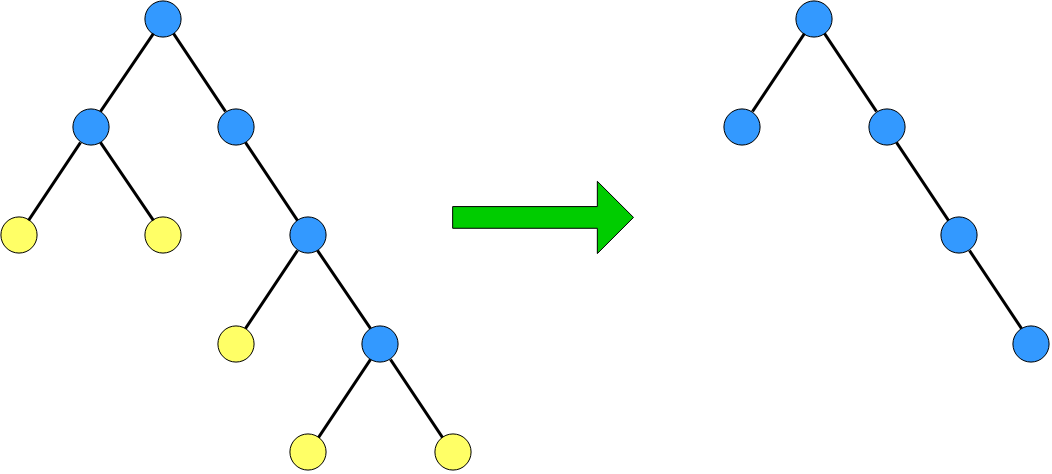
\includegraphics[width=0.8\textwidth]{pics/rake.png}
\caption{Операция Rake}
\label{pic:rake}
\end{figure}

Во время операции Compress выбирается некоторое множество несмежных друг с другом вершин.
Причем каждая такая вершина должна иметь ровно одного сына и при этом не быть корнем дерева. Чтобы выбрать такое множество применяется следующий метод.
Для каждой вершины с помощью генератора псевдослучайных чисел выбирается случайный бит. Вершина добавляется в множество, если у нее:
\begin{itemize}
\item ровно один ребенок;
\item она не является корнем;
\item биты, которые были сгенерированы для нее, ребенка и родителя, равны 0, 1 и 1 соответственно. 
\end{itemize}

Несложно заметить, что в выбранном таким способом множестве не будет смежных вершин.
Пример применения операции Compress показан на рис.~\ref{pic:compress}.

\begin{figure}[h]
\centering
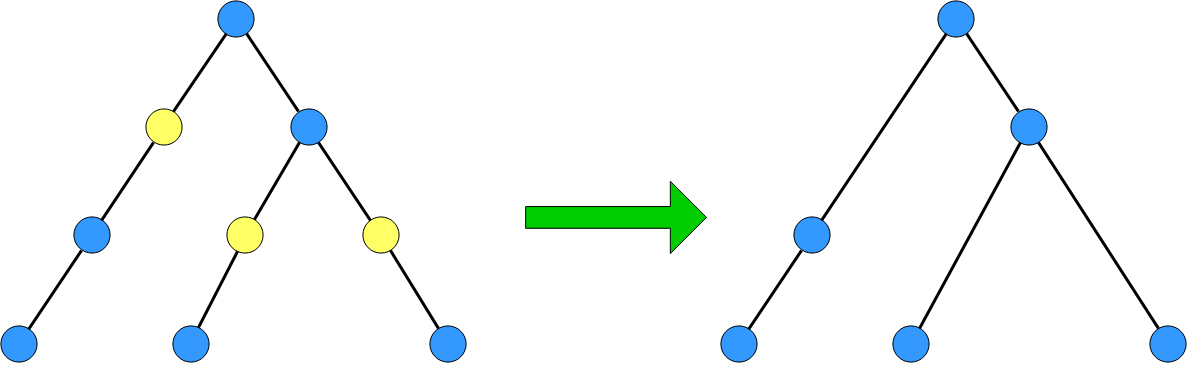
\includegraphics[width=0.8\textwidth]{pics/compress.png}
\caption{Операция Compress}
\label{pic:compress}
\end{figure}

Рассмотрим, как изменяется количество вершин в дереве, после применения к нему операций Rake и Compress. 
Разобьем все вершины дерева на три группы: входящая степень которых равна нулю, одному и больше одного. Обозначим их количество за $T_0$, $T_1$ и $T_2$ соответственно.
\begin{lemma}
\label{lem:cnt_vertices}
  $T_2 \leq T_0 - 1$
\begin{proof}
  Докажем по индукции по высоте дерева. 
  
  Для дерева из одной вершины утверждение верно. 
  
  Пусть утверждение доказано для деревьев высоты меньше $h$. Докажем для дерева высоты ровно $h$. 
  Рассмотрим степень корня. Если корень имеет ровно одного ребенка, то переходим к случаю дерева высоты $h - 1$. Если у дерева несколько поддеревьев, 
  то имеем 
  
  $T_2 = 1 + \sum\nolimits_{u \in children(root)} {T_2 (u)} 
             \leq 1 + \sum\nolimits_{u \in children(root)} {(T_0 (u) - 1)} \\
             \leq -1 + \sum\nolimits_{u \in children(root)} {T_0 (u)} 
             \leq -1 + T_0 = T_0 - 1$. 
  
  Заметим, что для леса деревьев лемма также справедлива.
\end{proof}
\end{lemma}

\begin{lemma}
\label{lem:const_factor}
После применения пары операций Rake и Compress к лесу, математическое ожидание количества вершин в нем не превосходит $\frac{7}{8}$ от их исходного числа.
\begin{proof}
Математическое ожидание количества удаленных вершин $deleted = T_0 + \frac{T_1}{8}$ 
(так как все листья будут удалены после операции Rake, а каждая вершина, у которой ровно один сын, будет удалена с вероятностью $\frac{1}{8}$ после операции Compress). 
Из леммы \ref{lem:cnt_vertices} получаем\\ $deleted = T_0 + \frac{T_1}{8} \geq \frac{1}{2} (T_0 + T_2) + \frac{1}{8} T_1 \geq \frac{1}{8} (T_0 + T_1 + T_2)$
\end{proof}
\end{lemma}
 
\begin{theorem}
\label{the:log}
 Математическое ожидание количества операций Rake и Compress, которые будут выполнены до полного сжатия дерева, равно $O(\log n)$, где $n$ --- общее количество вершин. 
\begin{proof}
Из леммы \ref{lem:const_factor} известно, что после каждой итерации применения операций Rake и Compress число вершин в среднем уменьшается в константное число раз. Значит, количество итераций в среднем ограничено $O(\log n)$.
\end{proof}
\end{theorem}

Из леммы \ref{lem:const_factor} также следует, что математическое ожидание суммарного числа вершин по всем итерациям равно $O(n)$. Это утверждение будет полезно для оценки количества используемой памяти.

\FloatBarrier
\section{Хранение Rake-Compress деревьев}
\label{sec:tree_storage}

Для того чтобы отвечать на запросы относительно структуры леса необходимо сохранить информацию о том, как происходил процесс сжатия леса. 
Будем хранить таблицу, в каждой строке которой будет записано состояние леса после применения операции Rake или Compress.
Каждый столбец таблицы будет соответствовать некоторой вершине. 
А каждая клетка будет хранить состояние некоторой вершины после какой-то итерации. Состоянием вершины будем считать ее родителя, а также множество детей. 
Если же вершина уже была сжата к этому моменту, то пометим это специальным образом. 

Пример такой таблицы показан на рис.~\ref{pic:table}. Рассмотрим более подробно процесс сжатия этого графа. 
Первоначальному состоянию дерева соответствует нижняя строка таблицы. После применения операции Rake к дереву, вершина 4 сжалась к своему родителю --- вершине 3.
Состояние дерева в этот момент сохранено во второй строке снизу. Например, в последнем столбце, который соответствует вершине номер 4, стоит прочерк, так как вершина была сжата к родителю.
После этого к дереву была применена операция Compress и вершина номер 2 сжалась к своему родителю. 
Заметим, что единственная вершина, которая могла быть сжата, во время операции Compress --- вершина номер 2, так как только у нее один ребенок, и она не явлется корнем дерева.
При этом на рисунке изображена ситуация, которая случится с вероятностью $\frac{1}{8}$, а с вероятностью $\frac{7}{8}$ после операции Compress данное дерево не изменится.
После этого произошла операция Rake, и в графе осталась только вершина с номером 1 --- корень дерева. 
Эта вершина будет удалена еще после двух итераций (операция Compress никак не изменит дерево из одной вершины).

\begin{figure}[h]
\centering
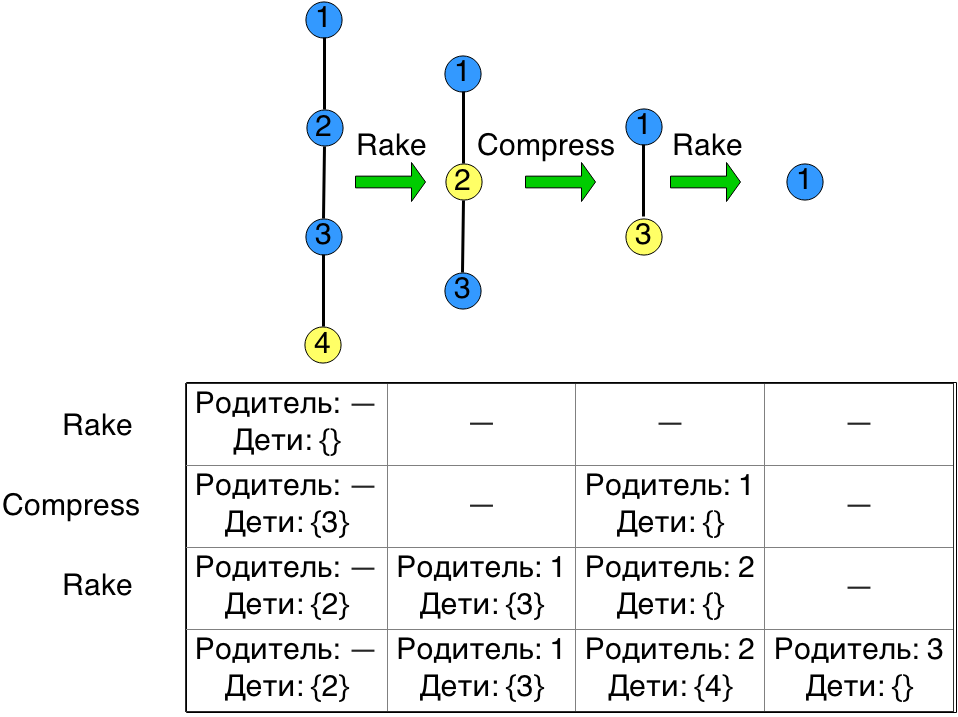
\includegraphics[width=0.8\textwidth]{pics/example.png}
\caption{Хранение Rake-Compress дерева в виде таблицы}
\label{pic:table}
\end{figure}


Из теоремы~\ref{the:log} известно, что математическое ожидание количества строк в такой таблице $O(\log n)$.  
Так как в таблице ровно $n$ столбцов, суммарное количество памяти, которое необходимо для хранение такой таблицы, равно $O(n \log n)$.
Если же в каждой строке хранить только существующие вершины с помощью ассоциативного массива, то количество используемой памяти уменьшится до $O(n)$. 
Однако, на практике использование ассоциативного массива оказывается нецелесообразным из-за большой константы.

\FloatBarrier
\section{Возможность параллельного построения}

Заметим, что операцию Rake и операцию Compress можно выполнять параллельно для всех вершин. 
Единственная часть алгоритма, которую непонятно как реализовать параллельно, является пересчет множества детей вершины при переходе к следующему слою. 
В оригинальной статье степень каждой вершины считалась константой, поэтому множества можно было хранить и пересчитывать любым способом. Если же предположить, 
что множество детей можно пересчитывать за $O(1)$, то Rake-Compress дерево можно построить за $O(\log n)$ в модели PRAM в случае наличия $\Omega(n)$ процессоров.

\FloatBarrier
\section{Ответ на запросы про структуру леса}

Рассмотрим, как с помощью таблицы, которая была описана ранее, отвечать на запросы. Самым простым запросом является ``определить корень дерева, в котором находится вершина $v$''.
Чтобы ответить на этот запрос необходимо проследить за вершиной $v$ в таблице. Будем переходить по строчкам таблицы начиная с первой. Если в некоторой строке нет клетки,
которая соответствует вершине $v$, то необходимо перейти к родителю вершины $v$ на предыдущей строке. Если же у нее не было родителя, то значит вершина $v$ является корнем.

Чтобы проверить, находятся, ли две вершины в одном дереве, необходимо найти корни деревьев, в которых находятся обе вершин и сравнить их.

Для ответа на более сложные запросы можно при сжатии вершины записывать в соответствующую клетку таблицы дополнительную информацию, а потом пользоваться ей. 
Заметим, что ответ на запрос происходит за время $O(\log n)$, так как на каждой строке таблицы тратится константное время.


\FloatBarrier
\section{Перестроение Rake-Compress дерева при изменении структуры леса}

Динамические Rake-Compress деревья основываются на следующей теореме.                                          

\begin{theorem}
Математическое ожидание количества клеток, которые поменяются в таблице Rake-Compress дерева при добавлении или удалении одного ребра из леса равно $O(\log n)$. 
Считается, что клетка поменялась, если поменялся родитель или множество детей.
Также, если клетка поменялась, то считается, что и все клетки, которые соответствуют этой вершине в более позднее время также поменялись.
\end{theorem}

Эта теорема доказана в оригинальной статье \cite{acar04} про Rake-Compress деревья. 
Хоть в самой статье авторы опираются на то, что степень каждой вершины ограничена константой, в конкретно этом доказательстве они этим не пользуются.

Таким образом, если научиться находить, а также пересчитывать значение, каждой из $O(\log n)$ изменившихся клеток за $O(1)$, то можно обрабатывать запросы добавления и удаления ребер за время $O(\log n)$.

\FloatBarrier
\section{Определение изменившихся клеток}
\label{sec:changed}
Рассмотрим, какие клетки таблицы Rake-Compress дерева изменяются при добавлении или удалении одного ребра в граф. 
Будем пересчитывать множество изменившихся клеток по индукции.
В первой строке таблицы изменились только клетки, которые соответствуют концам ребра.  
Если на некотором слое известно множество изменившихся клеток, то в это множество на следующем слое могут войти только вершины смежные с изменившимися.
В случае наличия ограничения на степени вершин, можно просто проверить все смежные вершины. Если же такого ограничения нет, то находить изменившиеся клетки необходимо иначе.

%В рассматриваемом случае необходимо действовать немного сложнее.
%Для этого будем честно определять, состояние каких вершин могло измениться. Необходимо рассмотреть моменты времени, когда вершина сжалась к своему родителю (как минимум в одной из версий).
%В любом случае, если вершина удаляется, то у нее не более двух соседей, которые и нужно пометить как изменившиеся. 

%Однако, после обнаружения, что клетка изменилась, необходимо также пересчитать ее состояние.
%В оригинальной статье говорится, что это можно сделать за константное время, так как количество детей ограничено.
%В нашем же случае нельзя пересчитывать состояние заново, поэтому необходимо узнать, как именно оно изменилось и поменять его за время пропорциональное количеству изменений.
%Однако, проблема состоит не только в сложности реализации, но и в том, что изменения необходимо внести и в клетки, которые соответствуют вершине в более поздний момент времени.
%Если хранить множества детей с помощью структуры данных, которая позволяет добавлять и удалять элементы за $O(1)$, то общее время обработки одного добавления или удаления ребра будет $O(\log^2 n)$.


\FloatBarrier

%-*-coding: utf-8-*-
\chapter{Оптимизация Rake-Compress деревьев}

В отличии от предыдущей главы, в данной главе рассматриваются деревья, у которых нет ограничения на степени вершин. 
В данной главе показаны новые методы, которые позволяют избавиться от этого ограничения, не увеличив при этом время работы.
Также в главе рассмотрены идеи, которые позволяют существенно уменьшить константу во времени работы и потребляемой памяти.
Кроме того, в данной главе показано, как можно использовать Rake-Compress деревья для пересчета функций на поддеревьях.

\FloatBarrier
\section{Определение и пересчет изменившихся клеток}
В разделе~\ref{sec:changed} показано, как находить клетки, которые поменялись в случае наличия ограничения на степени вершин дерева.
Существенное отличие заключается в том, что в общем случае нельзя проверить, изменились ли соседние вершины, так как их число может быть равно $\Omega(n)$.
Рассмотрим две таблицы Rake-Compress деревье для графов, которые отличаются одним ребром. Определим, чем отличаются эти таблицы.

Во-первых, отличаются клетки, которые соответствуют концам измененного ребра. 
Если же вершина не является концом ребра, то она будет считаться поменявшейся только в случае, если поменялось множество ее детей или родитель. 
А это может произойти только в том случае, если ее ребенком или родителем является поменявшаяся вершина и она сжалась к родителю хотя бы в одной из версий Rake-Compress таблицы.

Поэтому для каждой поменявшейся вершины будем следить, что с ней происходит в обоих версиях таблицы. 
Когда вершина сжимается к родителю, у нее может быть не более двух смежных вершин (включая родителя).
Значит, когда в какой-то из версий вершина удаляется, к множеству поменявшихся вершин нужно добавить $O(1)$ новых вершин.
Проблема заключается в том, что необходимо не только понять, что клетка поменялась, но и найти ее правильное состояние. 

Рассмотрим, например, случай, когда в ``старой'' версии таблицы вершина $v$ сжалась к вершине $p$ имея при этом единственного ребенка $c$. 
При этом из множества детей вершины $p$ удалилась $v$ и добавилась $c$, а новым родителем вершины $c$ стала вершина $p$. 
Если в ``новой'' версии такого сжатия не произошло, то необходимо вернуть все обратно --- из множества детей вершины $p$ удалить $c$ и добавить $v$, а родителем вершины $c$ назначить $p$.
Основная проблема заключается в том, что данные изменения необходимо сделать со всеми клетками, которые соответствуют вершинам $p$ и $c$ в более поздние моменты времени. А их может быть $\Omega(\log n)$.

Всего необходимо рассмотреть четыре случая (в зависимости от того, сжалась ли вершина в каждой из двух версий таблицы). 
В каждом таком случае необходимо отдельно обработать случаи, когда вершина является листом (у нее нет детей) или является корнем (у нее нет родителя).
Таким образом, рассмотрев большое количество случаев, можно получить алгоритм, 
который обрабатывает одно добавление или удаление ребра за время $O(\log^2 n)$, 
так как изменившихся клеток $O(\log n)$, а обработка каждой клетки занимает $O(\log n)$ времени (при условии, что добавление и удаление из множества детей происходит за $O(1)$).
\FloatBarrier
\section{Оптимизация памяти}
\label{sec:memory}

В разделе \ref{sec:tree_storage} говорилось, что Rake-Compress дерево принято хранить в виде таблице из $O(\log n)$ строк и $n$ столбцов. 
Суммарное количество непустых клеток $O(n)$, однако, их хранение с помощью ассоциативного массива, хоть и уменьшает асимптотику до $O(n)$, значительно увеличивает константу времени работы.
Поэтому на практике такой подход не используется. 

Предлагаемая оптимизация заключается в том, чтобы хранить таблицу по столбцам, а не по строкам. Каждый столбец соответствует некоторой вершине.
Заметим, что каждая вершина жива только первые несколько применений операций Rake и Compress. Если же в какой-то момент вершина была сжата к своему родителю, то далее она перестает быть живой.

Также следует отметить, что в случае изменения структуры леса, который хранится в Rake-Compress дереве, обращение часто происходит к клеткам из одного столбца. 
Если хранить дерево предложенным способом, эти обращения будут происходить к последовательным участкам памяти, что может положительно сказаться на производительности.

\FloatBarrier
\section{Хранение множества детей}
\label{sec:set_storage}

Рассмотрим более подробно, какие операции должна поддерживать структура данных, которая хранит в каждой клетке текущее множество детей вершины.
Ранее уже говорилось, что она должна поддердивать удаление и добавление элементов за $O(1)$. 
На самом деле множество детей хранится для того, чтобы определять, можно ли сжать вершину. Если детей у вершины больше одного, то ее точно нельзя сжать.
Если у нее нет детей, то ее можно сжать только во время операции Rake. Интересным являеися случай, когда у вершины ровно один ребенок. Тогда, чтобы определить 
можно ли приминить операцию Compress к вершине, нужно узнать, как бит был сгенерирован на текущей итерации для ребенка. А для этого необходимо знать, номер вершины-ребенка.
Значит, необходимо уметь определять, кто находится в множестве только в том случае, если в нем не более одного элемента.

Поэтому всю информацию о множестве можно хранить всего с помощью двух величин. А именно, можно хранить количество элементов в множестве и сумму их номеров. 
Тогда для добавления вершины в множество необходимо увеличить счетчик количества вершин, а также добавить к сумме номер вершины. 
Для удаления вершины из множества необходимо уменьшить счетчик количества вершин, и вычесть номер вершины из суммы. 
А когда в множестве останется ровно один элемент, то его номер будет равен сумме номеров всех элементов.

Данная оптимизация позволяет существенно уменьшить константу в асимптотике времени работы и используемой памяти. 

\FloatBarrier
\section{Пересчет состояний вершин в таблице Rake-Compress дерева}

Рассмотрим более подробно тонкости реализации Rake-Compress деревьев. В каждой клетке таблицы хранится состояние вершины в некоторый момент времени. 
В состояние вершин входит ее родитель, а также множество детей, которое хранится в виде суммы их номеров и их количества. Также будем запоминать, 
как изменяется состояние при переходе к следующему слою. А именно, будем хранить, кто должен стать новым родителем, на сколько изменится количество детей, а также как изменится сумма их номеров. 
Все это необходимо для того, чтобы обрабатывать каждую изменившуюся клетку за $O(1)$. 

Как только некоторая вершина помечается как изменившаяся, отменим ее действие на таблицу. 
А именно, найдем момент времени, когда вершина сжимается к родителю (если хранить таблицу по столбцам, это можно сделать за $O(1)$).
Рассмотрим, какие вершины поменяются при сжатии данной. Это ее родитель (если он есть), а также сын (если он есть).
Для каждой из этих вершин поменяем значения изменений, которые необходимо применить к состоянию. 
Также пометим, что эти вершины поменялись на этом слое. Для этого на каждом слое будем хранить список вершин, которые на нем поменялись. 
А перед тем как обрабатывать очередной слой будем добавлять в множество изменившихся вершин вершины из соответствующего списка. 

При этом необходимо удостоверится, что вершина еще не находится в множестве. 
Это можно сделать простых проходом по всему множеству (так как математическое ожидание количества вершин в нем равно константе).
Однако, есть и более эффективный с практической точки зрения метод. Будем считать, что к структуре данных поступают запросы о добавлении и удалении ребер. 
Тогда для каждой вершины будем запоминать номер последнего запроса, в котором вершина была помечена изменившейся. 
В таком случае можно будет узнать, лежит ли вершина в множестве изменившихся за одно обращение к массиву.

Кроме удаления эффекта от изменившихся вершин также необходимо и добавить правильный эффект. 
Для этого будем для каждой из изменившихся вершин определять, как ее состояние меняется при переходе к следующему слою.
Если вершина сжимается к ее родителю, то пометим родителя и ребенка (если он есть) и поменяем изменение, которое хранится в соответствующих клетках. 
А для пересчета состояния клеток воспользуемся значениями изменений, которые сохранены в клетках.
  
Таким образом, хранение изменений, которые должны произойти с клеткой при переходе к следующему слою, позволяет уменьшить время обработки одного запроса до $O(\log n)$. 

Реализация динаимических Rake-Compress деревьев на языке программирования Java доступна в \cite{github}.

\FloatBarrier
\section{Случай неориентированного дерева}
\label{sec:undirected}

Ранее был рассмотрен только случай корневых деревьев, однако Rake-Compress деревья можно строить и в неориентированном случае.
Операция Rake по-прежнему удаляет все листья дерева. А операция Compress применяется к вершинам, у которых ровно две смежные вершины. 
Предложенная оптимизация памяти также применима. А чтобы хранить множество вершин необходимо приложить чуть больше усилий.

Отличие неориентированного случая заключается в том, что необходимо узнавать номера смежных вершин в случае, когда их становится не больше двух. 
А, значит, хранить только сумму их номеров недостаточно. Поэтому предлагается кроме этого хранить сумму квадратов их номеров. Тогда, чтобы узнать, 
какие вершины принадлежат множеству необходимо будет решить квадратное уравнение.

\FloatBarrier
\section{Пересчет аддитивных функций}

Кроме запросов о структуре леса, Rake-Compress деревья можно использовать для подсчета значений некоторых функций. 
Например, каждой вершине можно сопоставить некоторое значение и узнавать, чему равна сумма значений всех вершин, которые находятся в поддереве.

Для этого в клетках таблицы Rake-Compress дерева необходимо хранить не только состояние вершины, но и значение функции, посчитанной на части дерева, которое уже было сжато в вершину. 
Если функция является аддитивной, то ее пересчет аналогичен пересчету множества детей вершины. 
Так, если некоторая вершина сжимается к родителю, то в соответствующей родителю клетке необходимо обновить значение функции. 
При добавлении и удалении ребер необходимо в изменившихся клетках пересчитывать значение функции. 
Аддитивность функции позволяет нам отменять сжатие вершины к своему родителю за $O(1)$. Поэтому общее время работы не изменится и будет составлять $O(\log n)$ на одно обновление.

Заметим также, что как и в случае с множеством детей, в каждой клетке необходимо хранить, как изменяется функция при переходе к следующему слою.

\FloatBarrier
\section{Пересчет ассоциативных функций}

Если же необходимо считать значение функции, которая не является аддитивной, то можно воспользоваться следующим методом.
В каждой клетке можно хранить все изменения функции, которые произошли из-за сжатия детей в виде сбалансированного двоичного дерева. 
Тогда при изменении множества детей, необходимо также соответствующим образом изменить дерево. 
Это приведет к тому, что в худшем случае пересчет таблицы Rake-Compress дерева при добавлении или удаления одного ребра будет работать за $\Theta(\log^2 n)$.


%%% Local Variables:
%%% mode: latex
%%% TeX-master: t
%%% End:
\chapter{Детали реализации и сравнение с аналогами}

В данной главе подробно рассмотрены детали реализации динамических Rake-Compress деревьев, а также приведен сравнительный анализ деревьев Rake-Compress и Link-Cut.

\FloatBarrier
\section{Генерация псевдослучайных бит}    
  
Для реализации Rake-Compress деревьев необходимо уметь генерировать случайные биты для определения, к каким вершинам можно применить операцию Compress.
Более формально, необходима структура данных, которая на вход принимает общее количество вершин и генератор псевдослучайных чисел, 
а на выход для каждой пары ($v$, $layer$) выдает случайный бит. 
При этом, для одинаковых входных данных, биты, которые генерируются, должны быть одинаковы вне зависимости от того, в каком порядке их спрашивают.
Также желательно чтобы данная структура данных занимала $O(n)$ памяти.

Воспользуемся оптимизацией, о которой говорится в разделе~\ref{sec:memory}. 
А именно, создадим генераторы псевдослучайных чисел для каждой вершины отдельно и будем отвечать на запросы лениво, сохраняя ответы в саморасширяющемся массиве (отдельном для каждой вершины).


\FloatBarrier
\begin{algorithm}
\caption{Структура данных для генерации случайных бит}\label{algo:random_gen}
\begin{algorithmic}[1]
\State $RandomBitsGenerator(int \ n, Random \ rnd)$
\For{$i = 0$ to $n$}
	\State $rand[i] \gets new \ Random(rnd.nextInt())$ 
	\State $bits[i] \gets \emptyset$
\EndFor

\Procedure{getBit}{$v, layer$}
	\While {$bits[v].size() \leq layer$}
		\State $bits[v].add(rand[v].nextBoolean())$
	\EndWhile
	\State \textbf{return} $bits[v].get(layer)$
\EndProcedure

\end{algorithmic}
\end{algorithm}

\FloatBarrier
\section{Хранение клеток таблицы Rake-Compress дерева}      

Рассмотрим более подробно, как необходимо хранить клетки таблицы Rake-Compress дерева. 
Для вершины необходимо сохранить ее родителя, а также множество детей. 
Как уже говорилось в разделе~\ref{sec:set_storage} множество детей хранится как сумма их номеров, а также их количество.
Если вершина является корнем, то в качестве ее родителя будем хранить ее номер.
Кроме того необходимо хранить изменения, которые произойдут с клеткой при переходе к следующему слою.

\FloatBarrier
\begin{algorithm}
\caption{Хранение клеток таблицы Rake-Compress дерева}\label{algo:cell}
\begin{algorithmic}[1]
\State \textbf{int} $id, parent, sumChild, cntChild$
\State \textbf{int} $newParent, diffSumChild, diffCntChild$

\Statex
\Procedure{applyChanges}{}
	\State $parent \gets newParent$
	\State $sumChild \gets sumChild + diffSumChild$
	\State $cntChild \gets cntChild + diffCntChild$
	\State $diffSumChild \gets 0$
	\State $diffCntChilde \gets 0$
\EndProcedure

\Statex
\Procedure{addChildToDiff}{$v$}
	\State $diffSumChild \gets diffSumChild + v$
	\State $diffCntChilde \gets diffCntChilde + 1$
\EndProcedure

\Statex
\Procedure{removeChildFromDiff}{$v$}
	\State $diffSumChild \gets diffSumChild - v$
	\State $diffCntChilde \gets diffCntChilde - 1$
\EndProcedure

\end{algorithmic}
\end{algorithm}

\FloatBarrier
\section{Хранение Rake-Compress дерева}   

Во-первых, для каждой вершины необходимо хранить список клеток, которые ей соответствуют. 
Кроме того, необходимо хранить генератор псевдослучайных бит. 
Также заведем счетчик количества примененных операций по изменению структуры леса.
Еще будем хранить массив, в котором для каждой вершины запишем номер последней операции, 
при обработки которой была изменена хотя бы одна клетка, которая соответствуют вершине.
Это позволит эффективно узнавать, была ли вершина уже помечена как поменявшаяся или нет.

\FloatBarrier
\begin{algorithm}
\caption{Хранение Rake-Compress дерева}\label{algo:rc_tree_storage}
\begin{algorithmic}[1]
\State $RakeCompressTree(int \ n, Random \ rnd)$
\State $RandomBitsGenerator \ rand \gets new \ RandomBitsGenerator(n, rnd)$
\State $time \gets 0$
\State $lastUpdateTime \gets \{0 ... 0\}$
\For{$i = 0$ to $n$}
	\State $cells[i] \gets new \ List<Cell>$ 
\EndFor

\end{algorithmic}
\end{algorithm}


\FloatBarrier
\section{Построение Rake-Compress дерева}   

Рассмотрим, как работает алгоритм построения Rake-Compress дерева. Будем строить таблицу по строкам.
В каждый момент будем хранить множество вершин, которые еще не были сжаты, и перестраивать следующий слой.
Также будем делать операции Rake и Compress одновременно. Чтобы определить, нужно ли сжимать вершину, 
воспользуемся следующим алгоритмом:

\FloatBarrier
\begin{algorithm}
\caption{Определение необходимости сжатия вершины}\label{algo:check_rake_compress}
\begin{algorithmic}[1]
\Procedure{shouldRemoveVertex}{$Cell \ c, RandomBitsGenerator \ rand, int \ layer$}
	\If {$c.cntChild = 0$}
		\State \textbf{return} \algorithmictrue \Comment{После применения операции Rake}
	\EndIf
	\If {$c.cntChild > 1$ \algorithmicor $c.parent = c.id$}
		\State \textbf{return} \algorithmicfalse
	\EndIf
	\If {$getCellForVertex(c.sumChild).cntChild = 0$}
		\State \textbf{return} \algorithmicfalse \Comment{Операция Rake была применена к ребенку}
	\EndIf
	\If {$rand.getBit(c.id, layer) = 0$ \algorithmicand $rand.getBit(c.sumChild, layer) = 1$ \algorithmicand $rand.getBit(c.parent, layer) = 1$}
		\State \textbf{return} \algorithmictrue
	\EndIf
	\State \textbf{return} \algorithmicfalse
\EndProcedure

\end{algorithmic}
\end{algorithm}

Общий алгоритм построения Rake-Compress дерева выглядит следующим образом:

\FloatBarrier
\begin{algorithm}
\caption{Алгоритм построения Rake-Compress дерева}\label{algo:building_rc}
\begin{algorithmic}[1]
\State $alive \gets \{0...n - 1\}$
\State $layer \gets 0$
\For{$i = 0$ to $n$}
	\State $cells[i].add(new \ Cell(parent[i]))$ 
\EndFor
\While {$alive \neq \emptyset$}
	\State $nextAlive \gets \emptyset$
	\For {$v \in alive$} 
		\State $c \gets getCellForVertex(v)$
		\If {$shouldRemoveVertex(c, rand, layer)$}
			\If {$c.cntChild = 1$}
				\State $getCellForVertex(c.sumChild).newParent \gets c.parent$
				\State $getCellForVertex(c.parent).addChildToDiff(c.sumChild)$
			\EndIf
			\If {$c.parent \neq v$}
				\State $getCellForVertex(c.parent).removeChildFromDiff(v)$
			\EndIf
		\Else
			\State $nextAlive.add(v)$
		\EndIf
	\EndFor
	\State $alive \gets nextAlive$
	\For {$v \in alive$}
		\State $newCell \gets getCellForVertex(v).clone().applyChanges()$ 
		\State $cells[v].add(newCell)$
	\EndFor
	\State $layer \gets layer + 1$
\EndWhile
\end{algorithmic}
\end{algorithm}

\FloatBarrier
\section{Изменение Rake-Compress дерева при удалении или добавлении одного ребра}   

Рассмотрим, что происходит с таблицей Rake-Compress дерева при изменении одного ребра.
Основная идея заключается в том, чтобы научится пересчитывать все изменения таблицы за время пропорциональное их количеству.
Для этого будем эффективно поддерживать множество изменившихся клеток. 
В момент, когда вершина помечается, как изменившаяся, найдем, как она влияет на таблицу и отменим это влияние. 
Для начала необходимо найти момент времени, когда вершина сжимается. В этот момент она влияет на не более чем две вершины. 
Изменим значения $cntChild$, $sumChild$ и $newParent$ нужным образом. 
Также необходимо добавить эти вершины в множество изменившихся (в момент, когда будет обработан соответствующий слой).
Поэтому для каждого слоя еще будем хранить список вершин, которые должны быть помечены перед обработкой слоя.

Алгоритм обновления дерева будет выглядеть следующим образом:


\FloatBarrier
\begin{algorithm}
\caption{Алгоритм перестроения Rake-Compress дерева при удалении или добавлении ребра}\label{algo:rebuilding_rc}
\begin{algorithmic}[1]
\State $time \gets time + 1$
\State $affected \gets \emptyset$
\State $markAffected(v)$ \Comment {Пусть ребро $(u, v)$ было удалено}
\State $markAffected(u)$
\State $cells[u].parent \gets u$
\State $cells[v].cntChild \gets cells[v].cntChild - 1$
\State $cells[v].sumChild \gets cells[v].sumChild - u$
\State $layer \gets 0$
\While {$affected \neq \emptyset$}
	\For {$v \in affectedOnLayer[layer]$}
		\State $markAffected(v)$
	\EndFor
	\For {$v \in affected$} 
		\State $c \gets getCellForVertex(v)$
		\If {$shouldRemoveVertex(c, rand, layer)$}
			\State $cells[v].size \gets layer + 1$
			\If {$c.cntChild = 1$}
				\State $getCellForVertex(c.sumChild).newParent \gets c.parent$
				\State $getCellForVertex(c.parent).addChildToDiff(c.sumChild)$
				\State $markAffected(c.sumChild)$
			\EndIf
			\If {$c.parent \neq v$}
				\State $getCellForVertex(c.parent).removeChildFromDiff(v)$
				\State $markAffected(c.parent)$
			\EndIf
			\State $affected \gets affected \setminus v$
		\EndIf
	\EndFor
	\For {$v \in affected$}
		\State $newCell \gets getCellForVertex(v).clone().applyChanges()$ 
		\State $cells[v][layer + 1] \gets newCell$
	\EndFor
	\State $layer \gets layer + 1$
\EndWhile

\Statex

\Procedure{markAffected}{$int \ v$}
	\If{$lastUpdateTime[v] = time$}
		\State \textbf{return} \Comment {Вершина уже помечена}
	\EndIf
	\State $lastUpdateTime[v] \gets time$
	\State $affected \gets affected \cup v$
	\State $removeEffectOfVertex(v)$
\EndProcedure
\Procedure{removeEffectOfVertex}{$int \ v$}
	\State $layer \gets cells[v].size()$
	\State $c \gets cells[v].get(layer)$
	\If {$c.parent = v$}
		\State \textbf{return}
	\EndIf
	\State $cells[c.parent].removeChildFromDiff(v)$
	\If {$c.cntChild = 1$}
		\State $cells[c.parent].addChildToDiff(c.sumChild)$
		\State $cells[c.sumChild].newParent \gets v$
	\EndIf
\EndProcedure

\end{algorithmic}
\end{algorithm}

\FloatBarrier
\section{Сравнение с Link-Cut деревьями}   

Алгоритм был реализован на языке программирования Java, с его исходным кодом можно ознакомиться в \cite{github}.
Был проведен сравнительный анализ производительности данного алгоритма, а также Link-Cut деревьев. 
В среднем на тестах, которые были проведены, Rake-Compress деревья оказываются медленнее в 5-10 раз чем Link-Cut.

Из этого можно сделать вывод, что в задачах, в которых применимы как Rake-Compress деревья, так и Link-Cut, следует использовать последние.
Однако, если в задаче требуется пересчитывать значения функций на поддеревьях, 
а не на путях, то Link-Cut деревья оказываются не применимы, и в таком случае можно воспользоваться Rake-Compress деревьями.
Кроме того, если удастся реализовать алгоритм, пересчитывающий Rake-Compress деревья и использующий несколько ядер одновременно, то, возможно, 
Rake-Compress деревья станут более востребованными.





\startconclusionpage

В данной работе была детально изучена структура данных Rake-Compress дерево. 
Она позволяет хранить информацию о лесе корневых деревьев и эффективно обрабатывать запросы его изменения (добавление и удаление ребер).

Реализация Rake-Compress деревьев, которая была описана в исходной статье, была существенно модифицирована. 
В частности, было показано как сократить расход памяти с $O(n \log n)$ до $O(n)$ без потери скорости работы.

Описанная в статье структура данных работала только в том случае, если степень каждой вершины ограничена некоторой константой. 
Было показано как избавиться от этого ограничения, не ухудшив время работы.

Также было показано, как применить предложенные оптимизации в случае неориентированных деревьев. 

Кроме того, был предложен способ пересчета функций на лесе деревьев. 
Для аддитивных функций пересчет осуществляется за время $O(\log n)$, а для ассоциативных за $O(\log^2 n)$.

Структура данных Rake-Compress дерево с предложенными оптимизациями была реализована на языке программирования Java. 
Было проведено сравнение данного алгоритма с алгоритмом Link-Cut дерева.

В дальнейшем планируется разработка алгоритма, который бы строил, а также перестраивал Rake-Compress деревья, используя несколько ядер одновременно.

\FloatBarrier


%\startappendices
%\label{appendix}
%\input{appendix}

\bibliographystyle{sty/utf8gost705u}
\bibliography{thesis}

\end{document}

%%% Local Variables:
%%% mode: latex
%%% TeX-master: t
%%% End:
